%-*- mode:latex; mode: auto-fill; mode: flyspell -*-
.\chapter{A survey of Cognitive Architectures}
\label{The_nature_of_cognition}
\newcommand{\soar}{{\small Soar\ }}
\newcommand{\actr}{{\small ACT-R\ }}
\newcommand{\epic}{{\small EPIC\ }}
\newcommand{\clarion}{{\small CLARION\ }}
The quest to understand the working of the human mind has spanned
many centuries starting with Plato when he asked, 
%
% as in the words of Noam Chomsky citing Bertrand Russell,
%
``{\bf How is it that human beings, whose contacts with the world are
  brief, personal and limited, are nevertheless able to know as much
  as they do?}''~\cite{Bogdan:1993aa}

Cognitive science brings together the varied disciplines of
psychology, neuroscience, computer science, linguistics and philosophy
in an attempt to answer the above question, using information
processing as a means to emulate the human mind. Psychology,
especially cognitive psychology, contributes theories on cognitive
capacities, information processing capabilities, sensory and motor
performance, and so forth.  Perhaps most importantly, it theorizes
about the overall picture of the human mind. Neuroscience, the study
of the brain and nervous system, provides a frame of reference against
which theories developed in cognitive science can be validated since
it deals with the brain at the lowest level.
% 
% Secondly, it provides knowledge for developing an alternative
% architecture of the mind. -- I was reffering to the connectionist
% architectures.
%
Computer science contributes knowledge representation, which is used
to develop theories to represent the way knowledge is stored,
artificial intelligence, which is used to analyse and create methods
for problem solving, and the theory of computation, which is used as a
means to understand foundational limits on cognition as
information processing.

The objective of this chapter is three-fold.  Firstly it aims to
provide a very brief introduction to human cognitive architectures
from both the cognitivist and emergent
perspectives~\cite{DBLP:journals/tec/VernonMS07}.  Secondly it
discusses cognitive architectures in general.  Finally it goes on to
compare some currently and widely used cognitive architectures.

\section{The nature of cognition}
\label{nature_Of_Cognition}
Any attempt to deal with the architecture of cognition has to answer
the following questions.

\begin{itemize}
\item \emph{What is knowledge and how can it be categorized?}  Since the aim
  of cognitive science is to understand the working of the human mind
  it is essential the nature of knowledge is understood because human
  beings function by processing information. Therefore it is
  imperative that we understand what knowledge is and the different
  forms of knowledge that are available.

  Although the nature of knowledge has been studied over many
  millennia we are still not certain of its characteristics.  For
  example, Brachman and Levesque~\cite{brachman-levesque:2004a}
  describe knowledge as a function that maps a ``knower'' to a
  proposition. A proposition is a statement that determines the truth
  value of the belief of the knower. But they also acknowledge that
  not all knowledge is of this form, for example, ``how to'' knowledge
  that enables someone to ride a bicycle.

\item \emph{How is knowledge acquired, represented and utilized?} When
  solving problems the human mind has the ability to retrieve and
  apply previously stored knowledge to the problem; for example,
  consider solving a calculus-based integration problem.  We are able
  to retrieve standard representations of the forms of equations and
  apply them to the problem to simplify it and solve it.  Issues of
  knowledge retrieval and application are central to understanding
  cognition.

\item {\em How do various processes act on this knowledge and how do
    they achieve the effect they intend to achieve?}  These two areas
  are significant because of their relationship to the techniques of
  deduction and inference that we use to solve problems on an everyday
  basis, inferences as simple and routine as when we diagnose a faulty
  light, or the more complex techniques we use when solving a
  crossword puzzle.

\item How can these processes and structures be manifested in the real
  world?  Purely theoretical accounts of cognition are important, but
  they must be validated by evidence that they can be realized by
  physical systems.  For scientists who study human cognition, this
  means ensuring that explanations of cognitive processing do not
  overstep the known limitations of the human brain and its
  processing.
\end{itemize}

These questions provide us with a very general framework for
understanding results produced in cognitive
science. Newell~\cite{Newell1980135} describes the study of the
working of the mind as a problem of satisfying the ``conjunction of
constraints on the nature of mind-like systems.'' He describes the
characteristics of what is to be expected of any theory that claims to
propose a model of human cognition. Newell mentions that this list is
not comprehensive, but in the view of Anderson and
Lebiere~\cite{CambridgeJournals:207162} it can used to provide a broad
framework against which all theories that claim to explain the human
mind can be tested.
 
The criteria listed below have been discussed in the
literature~\cite{CambridgeJournals:207162,Newell:1990aa}. The purpose
of listing them here is to explain as to what the study of the mind
would require.  A cognitive system must

\begin{itemize} 


\item {\em Behave flexibly as a function of the environment:} At first
  glance this statement may seem frivolous, as it seems to imply that
  human cognition functions in a haphazard manner. But Newell makes it
  clear that he is referring to the view that a cognitive system can
  be viewed as an instance of a universal computer, specifically a
  turing machine, despite its occasional failings and lack of infinite
  memory. He further explains that this view does not indicate the
  inablity to perform special operations, for example, vision. He
  explains that, like computers with special processing units, the
  cognitive system can be made up of special purpose systems that
  specialize in a certain task. As an example consider a chemist who
  can perform cognitive tasks in the laboratory---and who can also
  drive a car.

\item {\em Operate in real time:} A system that models cognition
  should be able to provide a plausible explanation for how humans are
  able to perform cognitive tasks at the rate they do. This criterion
  is important because otherwise a system could lead us to wrong
  assumptions about how humans think.

\item {\em Exhibit rational adaptive behaviour:} It must be able to
  explain this because humans perform computations, in the words of
  Newell\cite{Newell:1990aa}, are for ``the service of goals and
  rationally related to obtaining things that let the organism survive
  and propagate.''

\item {\em Display dynamic behaviour:} Humans operate in an
  environment that is ever changing. They draw in this information
  from their environment and act on it appropriately. For example, if
  you are driving a car and at some moment a deer decides to sprint in
  front of the car, you would hit the brakes.

\item {\em Integrate diverse knowledge:} Humans acquire knowledge from
diverse sources and are able to integrate them. For example consider a
computer programmer working in the banking industry. He can go to
school to obtain knowledge of the working of the finance industry. He
can use this knowledge along with his knowledge of computers science
to write programs for the industry. Here we see that our fictitious
programmer integrating knowledge, unlike expert systems where
knowledge is vertical and cannot be integrated as easily.

\item {\em Exhibits a sense of consciousness:} Newell does not point
  out the direct relation between consciousness and human cognition,
  but he mentions it as a criterion in his tests of human
  cognition. One interpretation~\cite{CambridgeJournals:207162} is
  that Newell is simply asking for the identification of cognitive
  properties that could support consciousness~\cite{Cohen:1996aa}

\item {\em Learning from the environment:} This point should be
  self-evident, we gain new knowledge from the world around us. But
  then the type of learning itself should be based on whether it can
  learn based on semantic memory, skill, priming and conditioning.

\item {\em Arise through evolution:} It is understood that the
  algorithms implicitly embodied by our cognitive processing are those
  that have arisen naturally over a period of time.  Hence any
  cognitive architecture should be able to learn and improve the
  algorithms through a process of improvement.

\item {\em Use of natural language:} Any theory that claims to
  decipher human cognition must be able to explain as to how we are
  able to comprehend what we listen to and understand what we say,
  because this is a function that is core to the way we communicate
  with each other.

\item {\em Be realizable with in the brain:} This point is critical
  because it serves as proof that a given theory is congruous with
  actual computations in the brain.

\end{itemize}

\section{Approaches towards explaining cognition}
There are many theories on the nature of cognition, each taking a
position on what constitutes cognitive functions and how they are
carried out. But these approches can be bifurcated into approaches
that adhere to the \emph{cognitivist
  approach}~\cite{DBLP:journals/tec/VernonMS07}, theories that view
cognition as information processes manipulating symbols, and those
that adhere to the \emph{emergent approach}, theories that treat
cognition as a process where models reflect the processes of cognition
by reorganization over time.

The goal of this section is to explore these disparate points of view
and to bring out differences between them.  We will then examine a
number of cognitive architectures in detail.

\subsection{The Cognitivist view}
     
The cognitivist perspective views human cognition as a set of
information processes working over a set of representations that point
to the actual knowledge which may be stored elsewhere, vis-\'{a}-vis
as symbols. These information processes are said to be purposeful,
contentful, representational, and can be described
formally\cite{103009}. Knowledge derived from these computations can
be stored and used later to improve the reasoning of the system. The
cognitivist view of perception is that it functions to generate an
appropriate representation of the the world around the system, which
the system can then reason about~\cite{DBLP:journals/tec/VernonMS07}.

The task of building models in cognitivist systems is generally done
by a programmer.  This has advantages, in that that these
representations and structures can be viewed and interpreted by
humans. But it may also bias the system, constraining it to an
idealized cognitive environment.  This causes problems when the system
has to stray away from its original requirements.  This gap between
perception, which is in interpretation of reality, and actual reality
begins to widen. This would then have to be filled in with more
programmer knowledge to close this ``semantic
gap''\cite{DBLP:journals/tec/VernonMS07}.
     
\subsection{The Connectionist approach}

     Until the 1980s the cognitivist viewpoint was the primary means
     of explaining the nature of human cognition. Interest in
     self-organizing systems led to an area of research that advocated
     the view that human cognition is made up of smaller units that
     rearrange themselves as the system acquires a skill or recognizes
     a change in its environment. This approach to understanding is
     known as the \emph{emergent approach}~\cite{DBLP:journals/tec/VernonMS07}.
     
     Although there are multiple methods are used to in the area of
     emergent systems, I will describe only connectionist view
     point. Connectionism is defined by Medler~\cite{Medler98abrief}
     as ``a theory of information that uses parallel processing of
     sub-symbols, using statistical properties instead of logical
     rules to transform information,'' rather than rules as used in
     classical cognitivist systems.

     The basic feature in a connectionist system is a 
     network. A connectionist network is made up of a number of simple
     computational units that communicate with each other with via
     connections. These connections are capable of carrying only
     simple information.
     
     The computational units in a connectionist system are arranged in
     a number of hierarchical layers.  Conventional systems include
     three types of layers: the input layer, at which input signals
     are set; the hidden layer or layers, which allow for combination
     of inputs; and the output layer. These networks can be arranged
     into two basic configurations, namely \emph{feed forward}
     networks and \emph{recurrent} networks.

     Feed forward networks(Fig \ref{ASCA_AFFN}) are those networks in
     which information flows in one direction only, that is, from the
     input layer to hidden layers (if they exist) and then to the
     output layer. Recurrent networks are those networks that have
     loops and hence backward connections.

     \begin{figure}[htp]
     \centering
     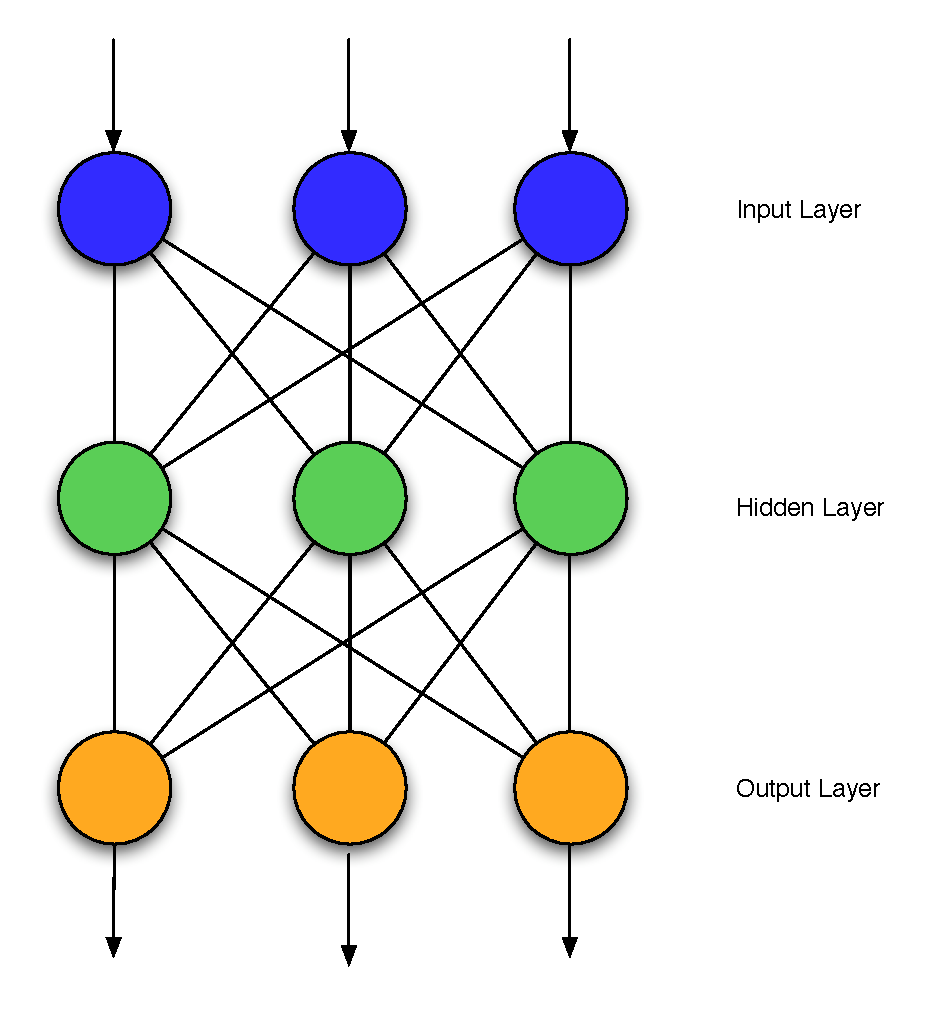
\includegraphics[width=80mm]{FeedForwardNetwork.eps}
     \caption{A feed forward network}
     \label{ASCA_AFFN}
     \end{figure}
     
     Connectionist models learn by adjusting the weights on the
     individual computational units. This implies that learning in
     connectionist models can be viewed more as a skill-building
     exercise, rather than an exercise in knowledge acquisition as in
     the case of the congitivist approaches~\cite{DBLP:journals/tec/VernonMS07}.
     
     The main attraction of connectionism is that it provides neural
     plausibility\cite{103009} to theories of cognitive science in its
     ability to simulate the massively parallel processing in the
     brain and in its ability to learn by adjusting weights. It is
     also attractive because it provides cognitive plausibility by
     allowing problems to be studied using simpler mechanisms. This
     can help in studying the processes underlying pattern-recognition
     and memory retrieval, as well as soft constraints for
     representing schematic knowledge.

     Despite these attractions, connectionist modelers find it
     difficult to explain the ability of the human mind to integrate
     diverse knowledge from various sources, the ability to use
     pre-existing knowledge, and the ability to respond in the time
     constraints that humans do.

     
\section{Cognitive Architectures}
% Talk about the need for cognitive architectures
Early work in psychology focused on producing micro theories, accounts
of highly constrained cognitive phenomena. Although each of these
micro theories explained its individual specialization well, there
were few attempts to integrate these in a complete picture of human
cognition~\cite{citeulike:4408336}.  Newell's work can be seen as a
call for cognitive scientists to provide a complete framework of human
cognition and to test theories of cognition within
it~\cite{Newell:1990aa, citeulike:4408336}.
%
Based on this we can define a cognitive architecture as

\begin{quote}
A framework that provides an interpretation of the working of
human cognition within which theories related to various aspects of
cognition can be validated based on that interpretation.
\end{quote}

% Explain the above definition more clearly
A basic view of human cognition is that of solving a constraint
satisfaction problem~\cite{Newell:1990aa}.  Cognitive science is still
a developing field and there can be numerous ways as to how these
constraints can be interpreted and solved by researchers.  Based on
this view, cognitive scientists are providing us with interpretations
of factors they believe constrain the way the mind works.
%
% SUN: He is explaining what the concept of architecture by providing
% an analogy to what architecture provides and things that can be
% moved around inside.
A cognitive architecture provides us with an invariant environment
where we can perform detailed modeling that helps us in understanding
the processes, structures and the organization between these
structures in the brain\cite{journals/jetai/Sun07}.

% List out the uses of cognitive architectures
Sun~\cite{journals/jetai/Sun07} describes the significance of the study
of cognitive architectures as follows.
\begin{itemize}
\item They provide a means of understanding cognition.
\item They provide a foundation to build intelligent systems that are
  cognitively realistic.
\end{itemize}

We will now discuss criteria for comparing cognitive architecture and
we will also look at some sample cognitive architectures.

% Define and explain what is needed from a cognitive architecture.
\section{Survey of cognitive architectures}

In this section I will describe a number of popular cognitive
architectures that are currently in use. I will later compare them
based on a number of criteria that reflect the functions that a
congitive architecture is supposed to perform.

% General template
% Describe architecure
%   Knowledge representation, 
%      short term memory, long term memory, Goals,
%   Mechanics of cognition
%      Means of planning, Learning
%   Abilities of perception
%      Auditory, Visual

\subsection{ACT-R}

\begin{figure}[htp]
  \centering
  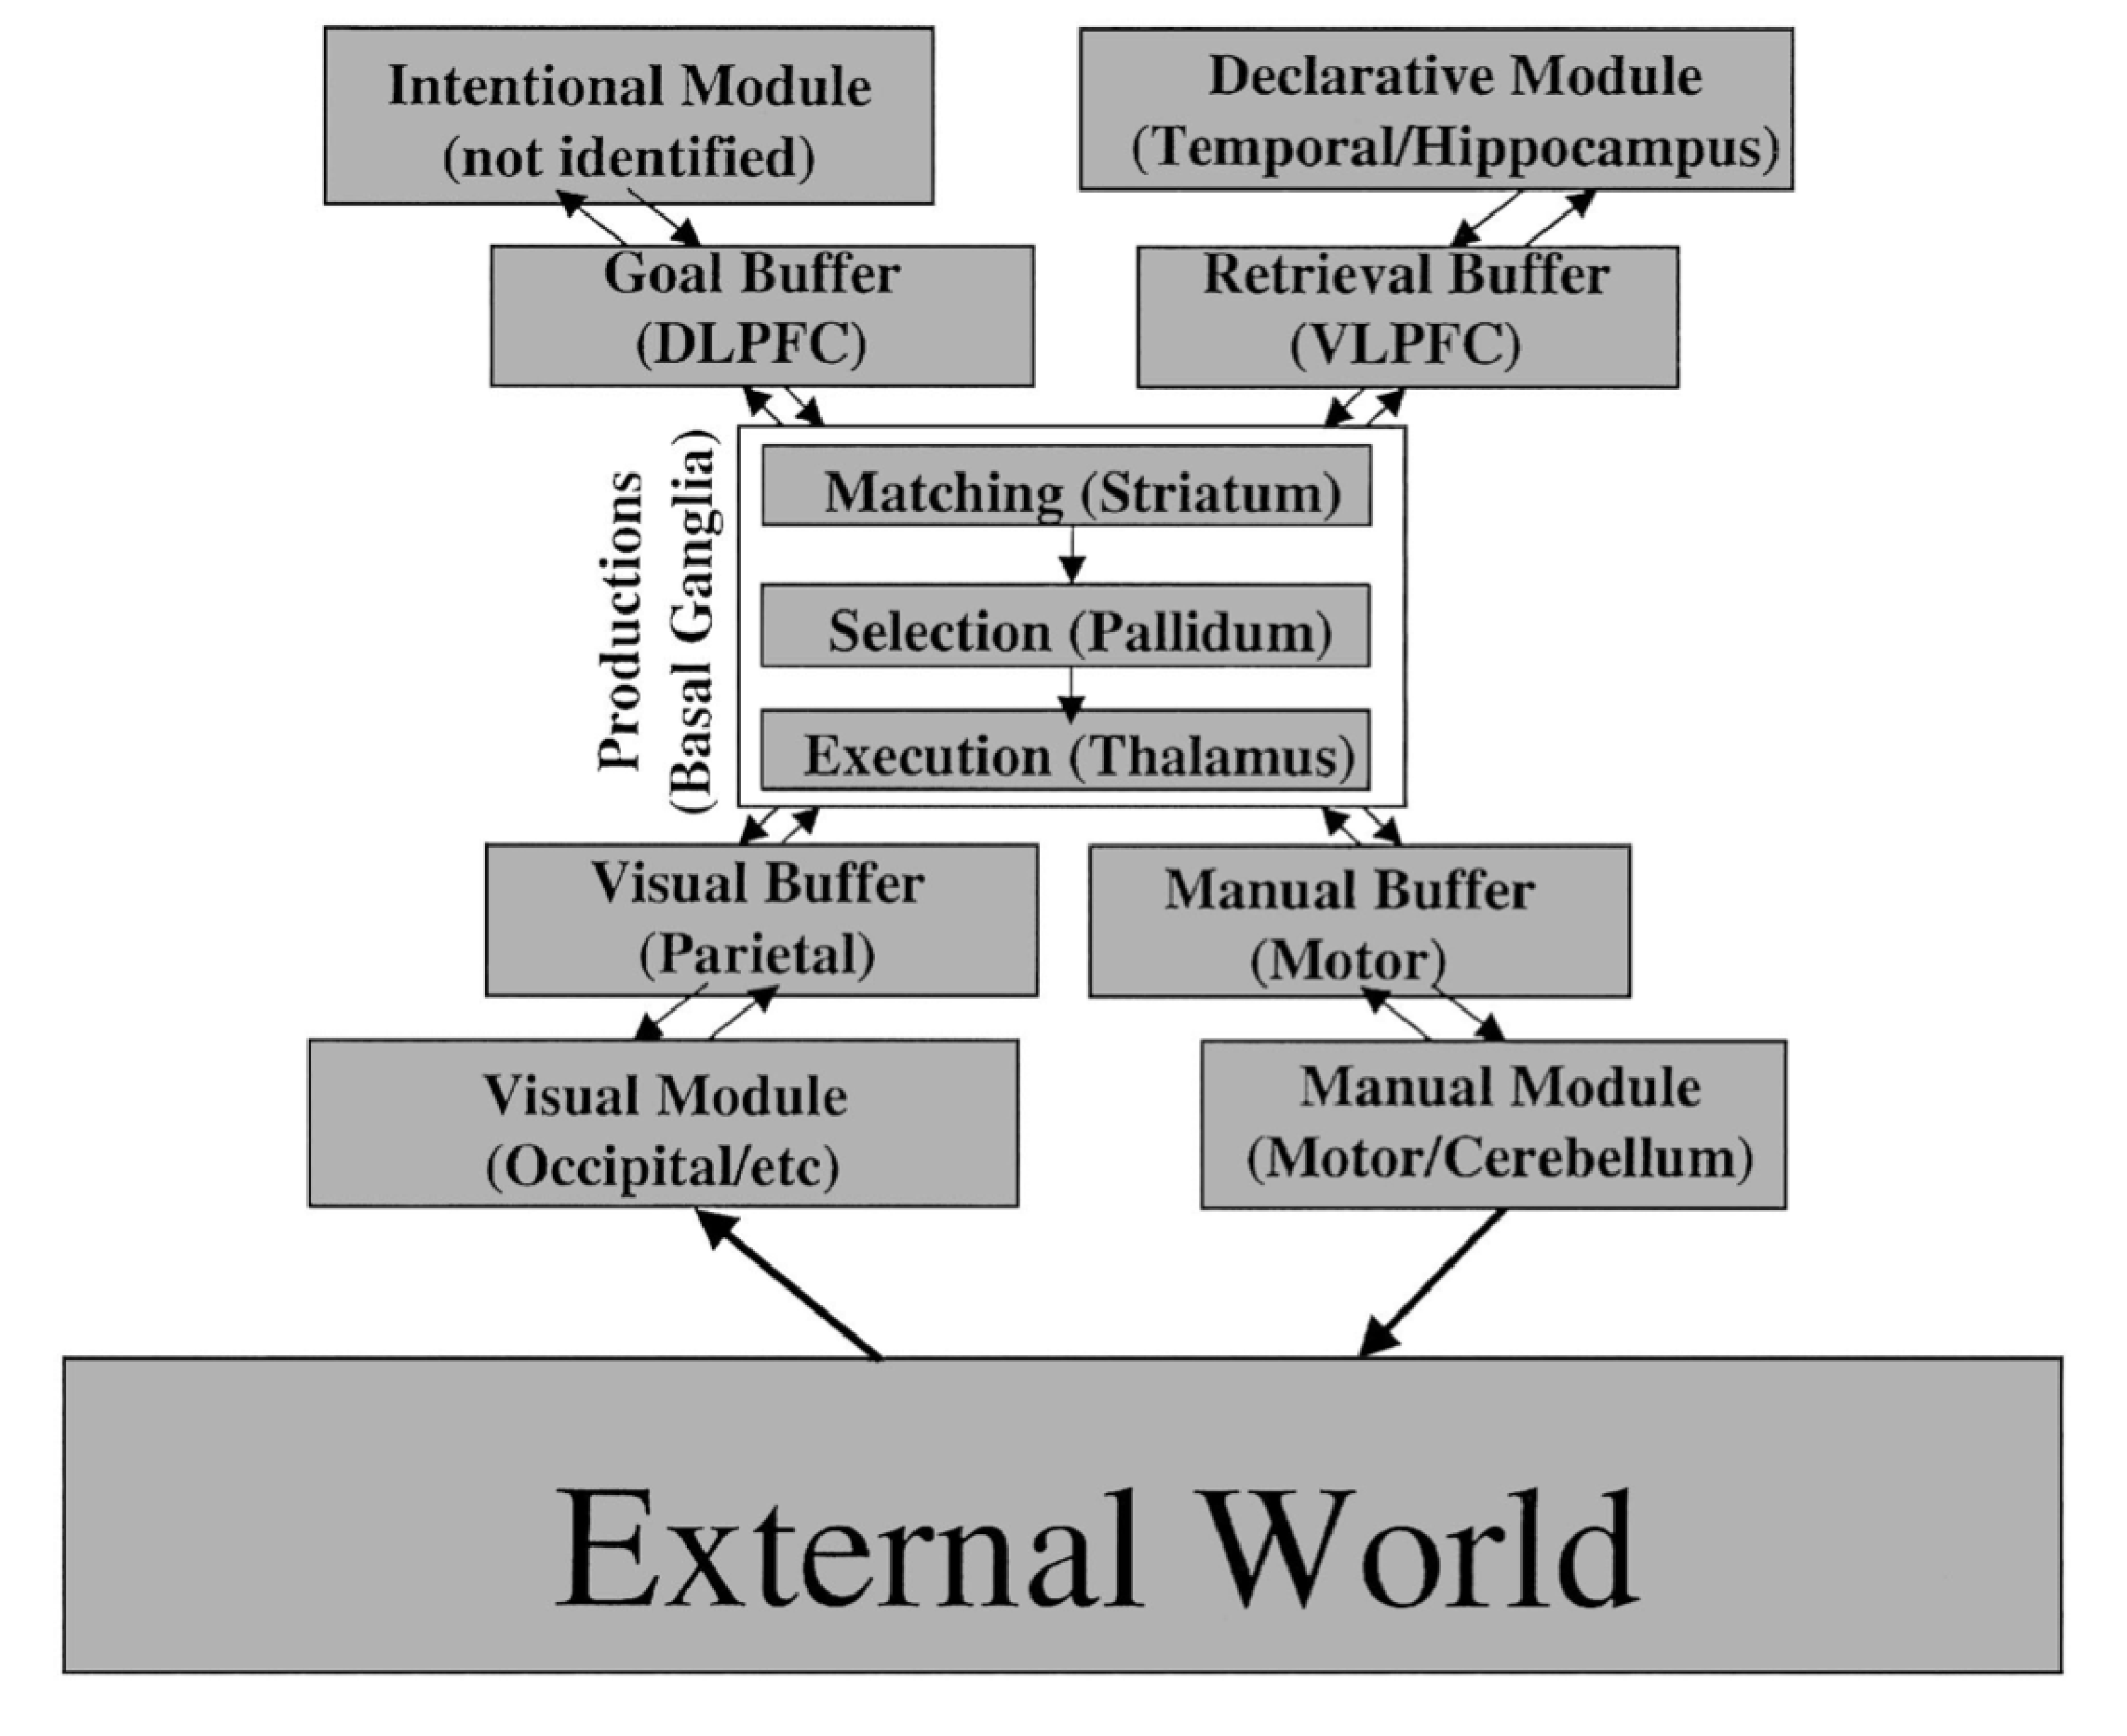
\includegraphics[width=100mm]{ACTRArch.eps}
  \caption{The architecture of ACT-R 5.0\cite{anderson_jr-etal:2004a}}
  \label{ACTR_ARCH}
\end{figure}


% Describe architecure

% Architecture Background
\actr was developed by Anderson et al.~\cite{anderson_jr-etal:2004a}
at Carnegie Mellon University to validate results performed by in the
area of cognitive psychology. \actr's origins lie in an attempt by
Anderson and Bower to describe a theory that explained the working of
memory called Human Associative Memory(HAM)\cite{AndersonBower73}. HAM
eventually grew into {\small ACT}\cite{Anderson76} which in due course evolved
into \actr\cite{Anderson83}.

% Describe the architecture given in the picture.
ACT-R consists of a set of core modules. These modules aim to
represent constituent functions of the brain. The operation of these
modules is coordinated by a central production system. This system can
identify patterns and make changes to the contents of buffers. The
organization of these modules can be seen in figure \ref{ACTR_ARCH}. I
describe each of these modules below.

\begin{itemize}
\item {\bf Visual Module}: This module provides ACT-R with the capability of
  identifying objects visually.
\item {\bf Manual Module}: This module provides ACT-R with the ability to
  perform motor actions.
\item {\bf Intentional Module}: This module helps ACT-R simulate the
  ability to keep track of current goals.
\item {\bf Retrieval Module}: This module implements the mechanism to
  retrieve chunks of information from the declarative memory.
\end{itemize}

%   Knowledge representation, 
%      short term memory, long term memory, Goals,
In ACT-R information stored in human memory such as phone numbers and
words are stored in chunks. Chunks can either be declared at the start
of the model or are created during the execution of the model. Chunks
represent information in the declarative memory of the architecture. The
probability and the speed with which a chunk might be retrieved is
controlled by its activation. This is defined by the equation
%
\begin{equation}
  A_i = B_i + \sum_j W_j S_{ij},
\end{equation}
%
where $A_i$ is the activation level of the chunk, $B_i$ is the base
level activation of the chunk, $W_j$ is the attentional weighting of
the elements of the current goal, and $S_{ij}$ represents the strengths
of associations from elements $j$ to chunk $i$.

%   Mechanics of cognition
%      Means of planning, Learning
The production system controls the coordination between various
modules.  This is done through selecting the appropriate production
and firing it. Though there may be a number of competing productions,
the single production with the highest utility is selected.  The
utility of a production is defined by
%
\begin{equation}
  U_i = P_iG - C_i,
\end{equation}
%
where $P_i$ is the probability that the production $i$ will achieve
the goal $G$.  $C_i$ defines the cost of completing the goal. This is
estimated by the amount of time left to complete the goal.

ACT-R learns through a process of production compilation
\cite{oai:CiteSeerPSU:518586}. It attempts to teach successive pairs
of productions and tries to unify them into a single production. But
this is not a complete explanation; it breaks down when the
productions consist directives to the visual-motor modules.

%   Abilities of perception
%      Auditory, Visual, Motor
% The motor perceptual system
% The act-r motor perceptual system is essentially borrowed of the
% EPIC system.

The ACT-R motor-perceptual system is modeled after EPIC
(executive-process/interactive-control)~\cite{kieras1997overview}. The
perception of vision is provided by the visual module, which itself
consists of two modules, the visual-location module and visual-object
module. The visual-location module helps the visual module to focus
its attention to a location in the visual field specified by the
buffer. The visual-object module holds information about the object in
the visual field. Motor control is provided by the manual
module. ACT-R also has rudimentary auditory and vocal
modules\cite{anderson_jr-etal:2004a}.

% The approach taken was to model the basic timeing behaviour of those
% systems in an approximate form. The model the timing behaviour,
% input and output behaviours.

\subsection{Soar}

% Describe architecture background
\soar is a general cognitive architecture proposed originally by Allen
Newell~\cite{Newell:1990aa,27702}, when he argued for the need for
psychology to deal with human cognition as a whole, rather than in
form of micro strategies. The major ideas\cite{Lewis:2001aa, 27702} that
define the characteristics of \soar are these:

% Describe the motivations behind SOAR, the technical ideas that
% constitute 
\begin{itemize}
\item \emph{Physical symbol system hypothesis} : General intelligence
  can be realized with a symbolic system\cite{Newell1980135}.
\item \emph{Goal structure hypothesis}: Control of general
  intelligence is maintained by a symbolic goal system.
\item \emph{Uniform elementary-representation hypothesis}: There is a
  single representation for declarative knowledge.
\item \emph{Problem space hypothesis}: problem spaces are the
  fundamental organizational unit of all goal directed behaviour.
\item \emph{Production system hypothesis}: Production systems are the
  appropriate encoding for long term knowledge.
\item \emph{Universal sub-goaling hypothesis}: Any decision can be an
  object of goal-oriented attention.
\item \emph{Automatic sub-goaling hypothesis}: All goals arise
  dynamically in response to impasses and are generated automatically
  by the architecture.
\item \emph{Control-knowledge hypothesis}: Any decision can be
  controlled by indefinite amounts of knowledge that can be either domain-
  dependent or independent.
\item \emph{Weak-method hypothesis}:  Weak methods form the basic
  methods of intelligence. % $<$\textsc{Do a bit of background reading$>$}.
\item \emph{Weak-method emergence hypothesis}:  Weak methods arise
  directly from the system responding to its environment based on its knowledge of the
  task.
\item \emph{Uniform learning hypothesis}: Goal-based chunking is the
  general learning mechanism.
\end{itemize}
%   Knowledge representation, 
%      short term memory, long term memory, Goals,
According to the \soar theory, human memory is composed to two
separate memories: long term memories stores information for a long
period of time, and working memory stores information required for the
task currently at hand.

Long term memory (LTM) stores information that can be applied a number
of instances of tasks. LTM is composed of three memories: procedural
memory, semantic memory, and episodic memory. Procedural memory stores
information about how a task is supposed to be carried out, for
example it would store information about tasks such as changing a
light bulb, looking up a word in the dictionary, even eating
breakfast.  Semantic memory is used to store information related to
facts about the environment in which the agent operates.  For example,
an agent tried to decide what to eat for breakfast knows the kinds of
food that are generally eaten at that time of day.  Episodic memory
stores information about specific incidents along with contextual
information.  For example, the breakfast-choosing agent might recall
information from episodic memory about what it had for breakfast
yesterday.  Information stored in the procedural memory is accessed
more frequently than information from either the semantic or episodic
memories, because this information directly controls the behavior of
the agent.

All information in the LTM is stored in the form of
\emph{productions}. A production consists of a set of conditions and a
set of corresponding actions. Productions provide control information
for the application of operators on a candidate state in  working
memory. Productions perform four different roles: three knowledge
retrieval problem solving functions and a state elaboration
function. The knowledge retrieval functions are operator proposal,
operator comparison, and operator
application~\cite{Laird:2006aa}. Productions in \soar are fired in
parallel without conflict resolution (unlike \actr, which has a
conflict resolution mechanism to select between competing
productions).

\emph{Preference Memory} is used to decide which operator is the best in the
given circumstance.  Preferences in the memory are used to compare a
selected set of operators with one another in an attempt to pick 
the best operator. Actions in productions are instrumental in creating
productions. These remain active as long as the production is deemed
suitable for the situtation and are removed once the production is no longer
valid.

\emph{Working Memory} (WM) describes memory that hold information
related to the task that is currently being executed. This includes
states and sub-states created to solve the problem, operators that are
applicable to the current states and Working Memory Elements (WME)
that hold specific information about a specific identifier. Elements
in working memory are created by the action of productions, a state
created as a result of an \emph{impasse}, or because of the action of
external I/O systems. Information from the working memory is removed
only when it becomes irrelevant to the existing situtation. This
architecture can be seen in figure \ref{SOAR_ARCH}.

\begin{figure}[htp]
  \centering
  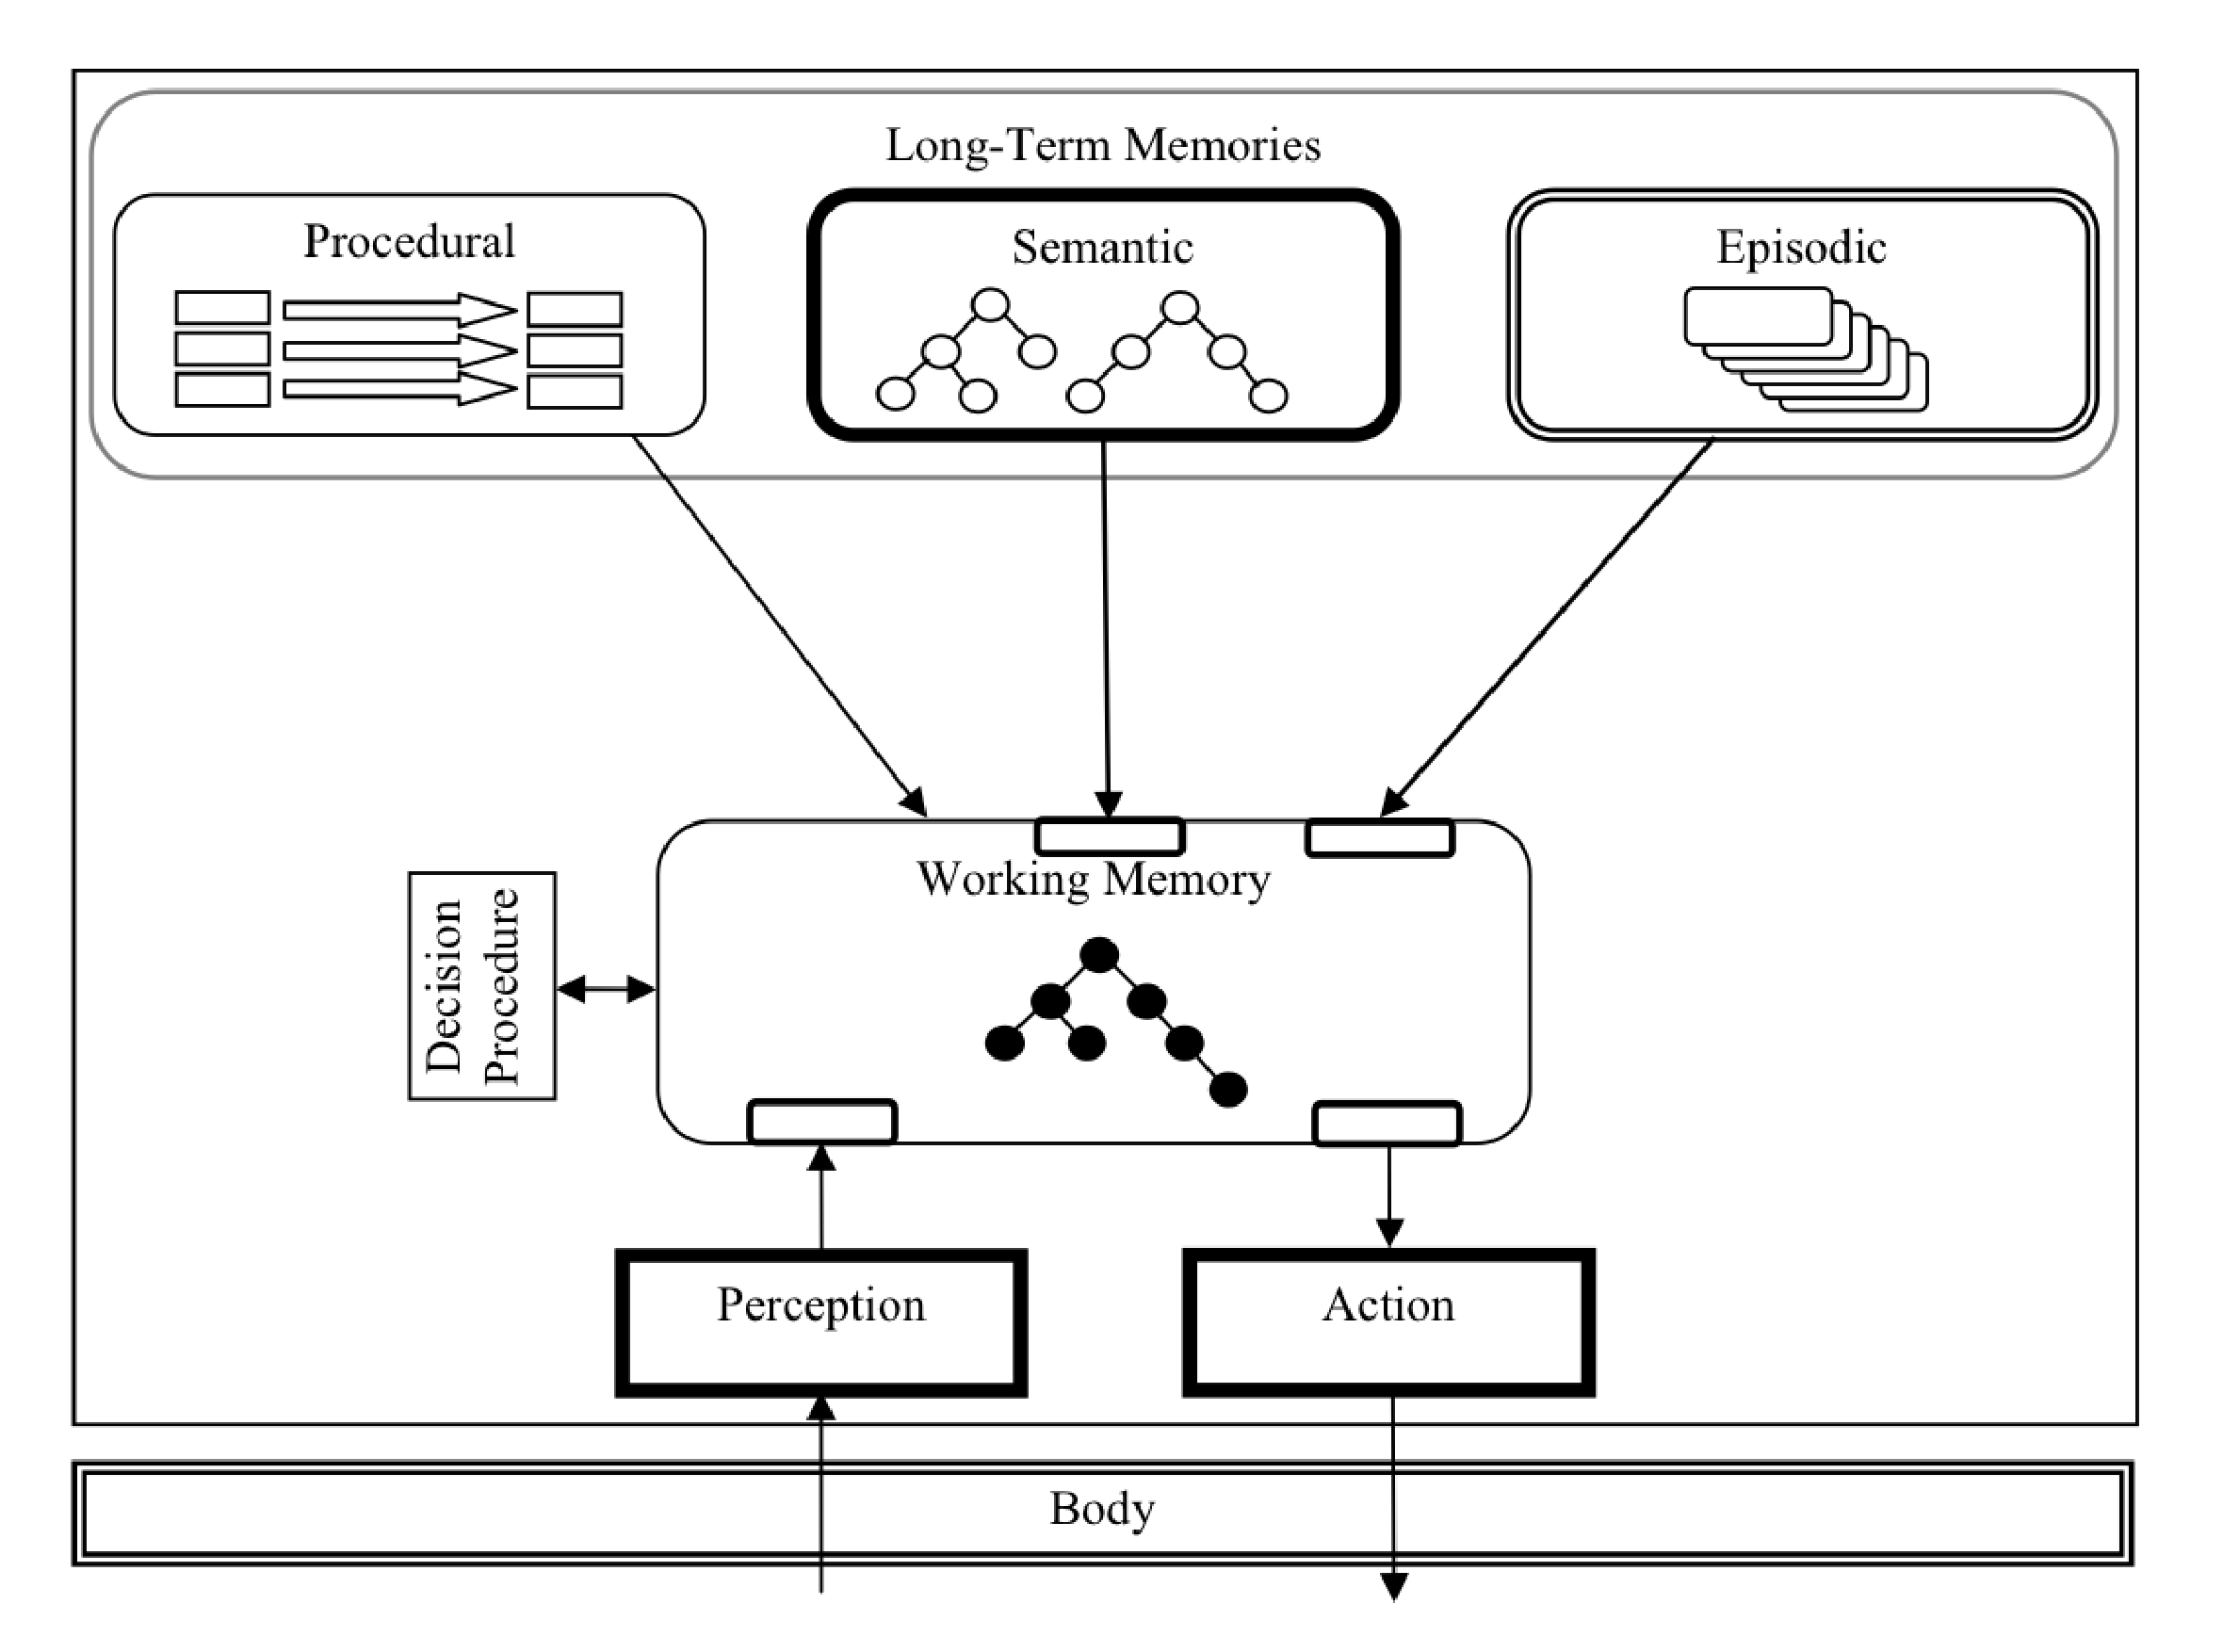
\includegraphics[width=100mm]{soar.eps}
  \caption{Soar Architecture\cite{Jill-Fain-Lehman:2006aa}}
  \label{SOAR_ARCH}
\end{figure}

%   Mechanics of cognition
%      Means of planning, Learning
% Describe searching in a space, impasses, subgoaling, creation of new states
The \soar theory maintains that cognition is flexible and goal-driven,
that learning is a continuous process that arises from experience. This assumption
is realized as a search in a problem space supported by a
\emph{recognize-decide-act} control structure\cite{Lewis:2001aa}. The
{\em recognize} phase consists of firing all productions that are relevant
to the phase, which results in addition of new content to the working
memory. The {\em decide} phase makes a decision about what the system should
do next. If all the processes of the decide step converge to a
decision, then that decision is placed in the working memory with the
assertion that this decision would be the next step. The {\em act} phase
involes actually realizing the step. 
% Give an overview of chunking
 
During the decision phase it is possible that the
preferences might be incomplete or inconsistent. Such a situation is
called an \emph{impasse}. In the event that an impasse is detected, a
substate of the current state is created whose goal is to resolve the
inconsistency. New productions are produced as a result of this
problem-solving activity. The conditions of the new productions
consist of information about the the state of working memory before the
impasse; the actions consist of  new information obtained from
resolving the impasse. If a similar situation is encountered in the
future, the conditions are matched and the corresponding actions are
executed.  This process is called \emph{chunking}.  This is how
\soar obtains knowledge when solving a specific problem.
%   Abilities of perception
%      Auditory, Visual

% $<$ \textsc{The \soar architecture does not describe its perceptual
%  motor facilities in detail. What do I write about that?} $>$
% RSA: Soar doesn't have any built-in perceptual/motor capabilities.

% Give a general over view of the input and output capabilities

\subsection{EPIC}
% Describe architecure
The Executive-Process/Interactive-Control(\epic)
system~\cite{kieras1997overview} attempts to take on the challenge of
developing a theory for cognition from a different perspective. The
\epic architecture maintains that human cognition is constrained by the
physiological aspects of the human rather than its cognitive
machinery. The motivations for developing this architecture are

\begin{itemize}
\item \emph{To analyze a cognitive system that is tied closely to its
    perceptual-motor faculties}: Most cognitive architectures around
  the time when \epic was developed represented human cognition as
  being \emph{disembodied}. They represented cognition as a system that
  perceived the environment and directly acted on it without
  considering the limitation and interactions between of intermediate
  perceptual-motor systems and the cognitive systems.
\item \emph{Study models that simulated both performance and
    cognition}: Kieras and Meyer were interested in studying the field of
  human attention and performance from the computational modeling
  paradigm and hence to further the state of this psychological theory.
\item \emph{Study the role of executive processes and performance in
    environment that require execution of multiple tasks}: From the
  cognitive modeling perspective, an executive process is one that
  controls all other cognitive processes. Kieras and Meyer intended to
  study this aspect of cognition. They assert that the best way to do
  so is to study human performance in a environment that entails
  execution of multiple tasks, and that human cognitive capability is
  constrained only by the physical limitations.
\end{itemize}
% Motivation

%   Knowledge representation, 
%      short term memory, long term memory, Goals,
The architecture of \epic is shown in figure \ref{EPIC_ARCH}.
% $<$ \textsc{Think of a better way to start this paragraph}.
%
The \epic architecture uses separate memories to store procedural
information, such as production rules and separate memory to store
formal knowledge. The working memory consists of two 'amodal' types of
information.  One stores control information such as information
pertaining to goals and steps with in the current procedure. The
second memory is called {\em general WM} and is used to store
miscellaneous task information. The \epic architecture does not make
any assumptions about decay, capacities, or representational
properties of the working memory\cite{citeulike:3439185}.

\begin{figure}[htp]
  \centering
  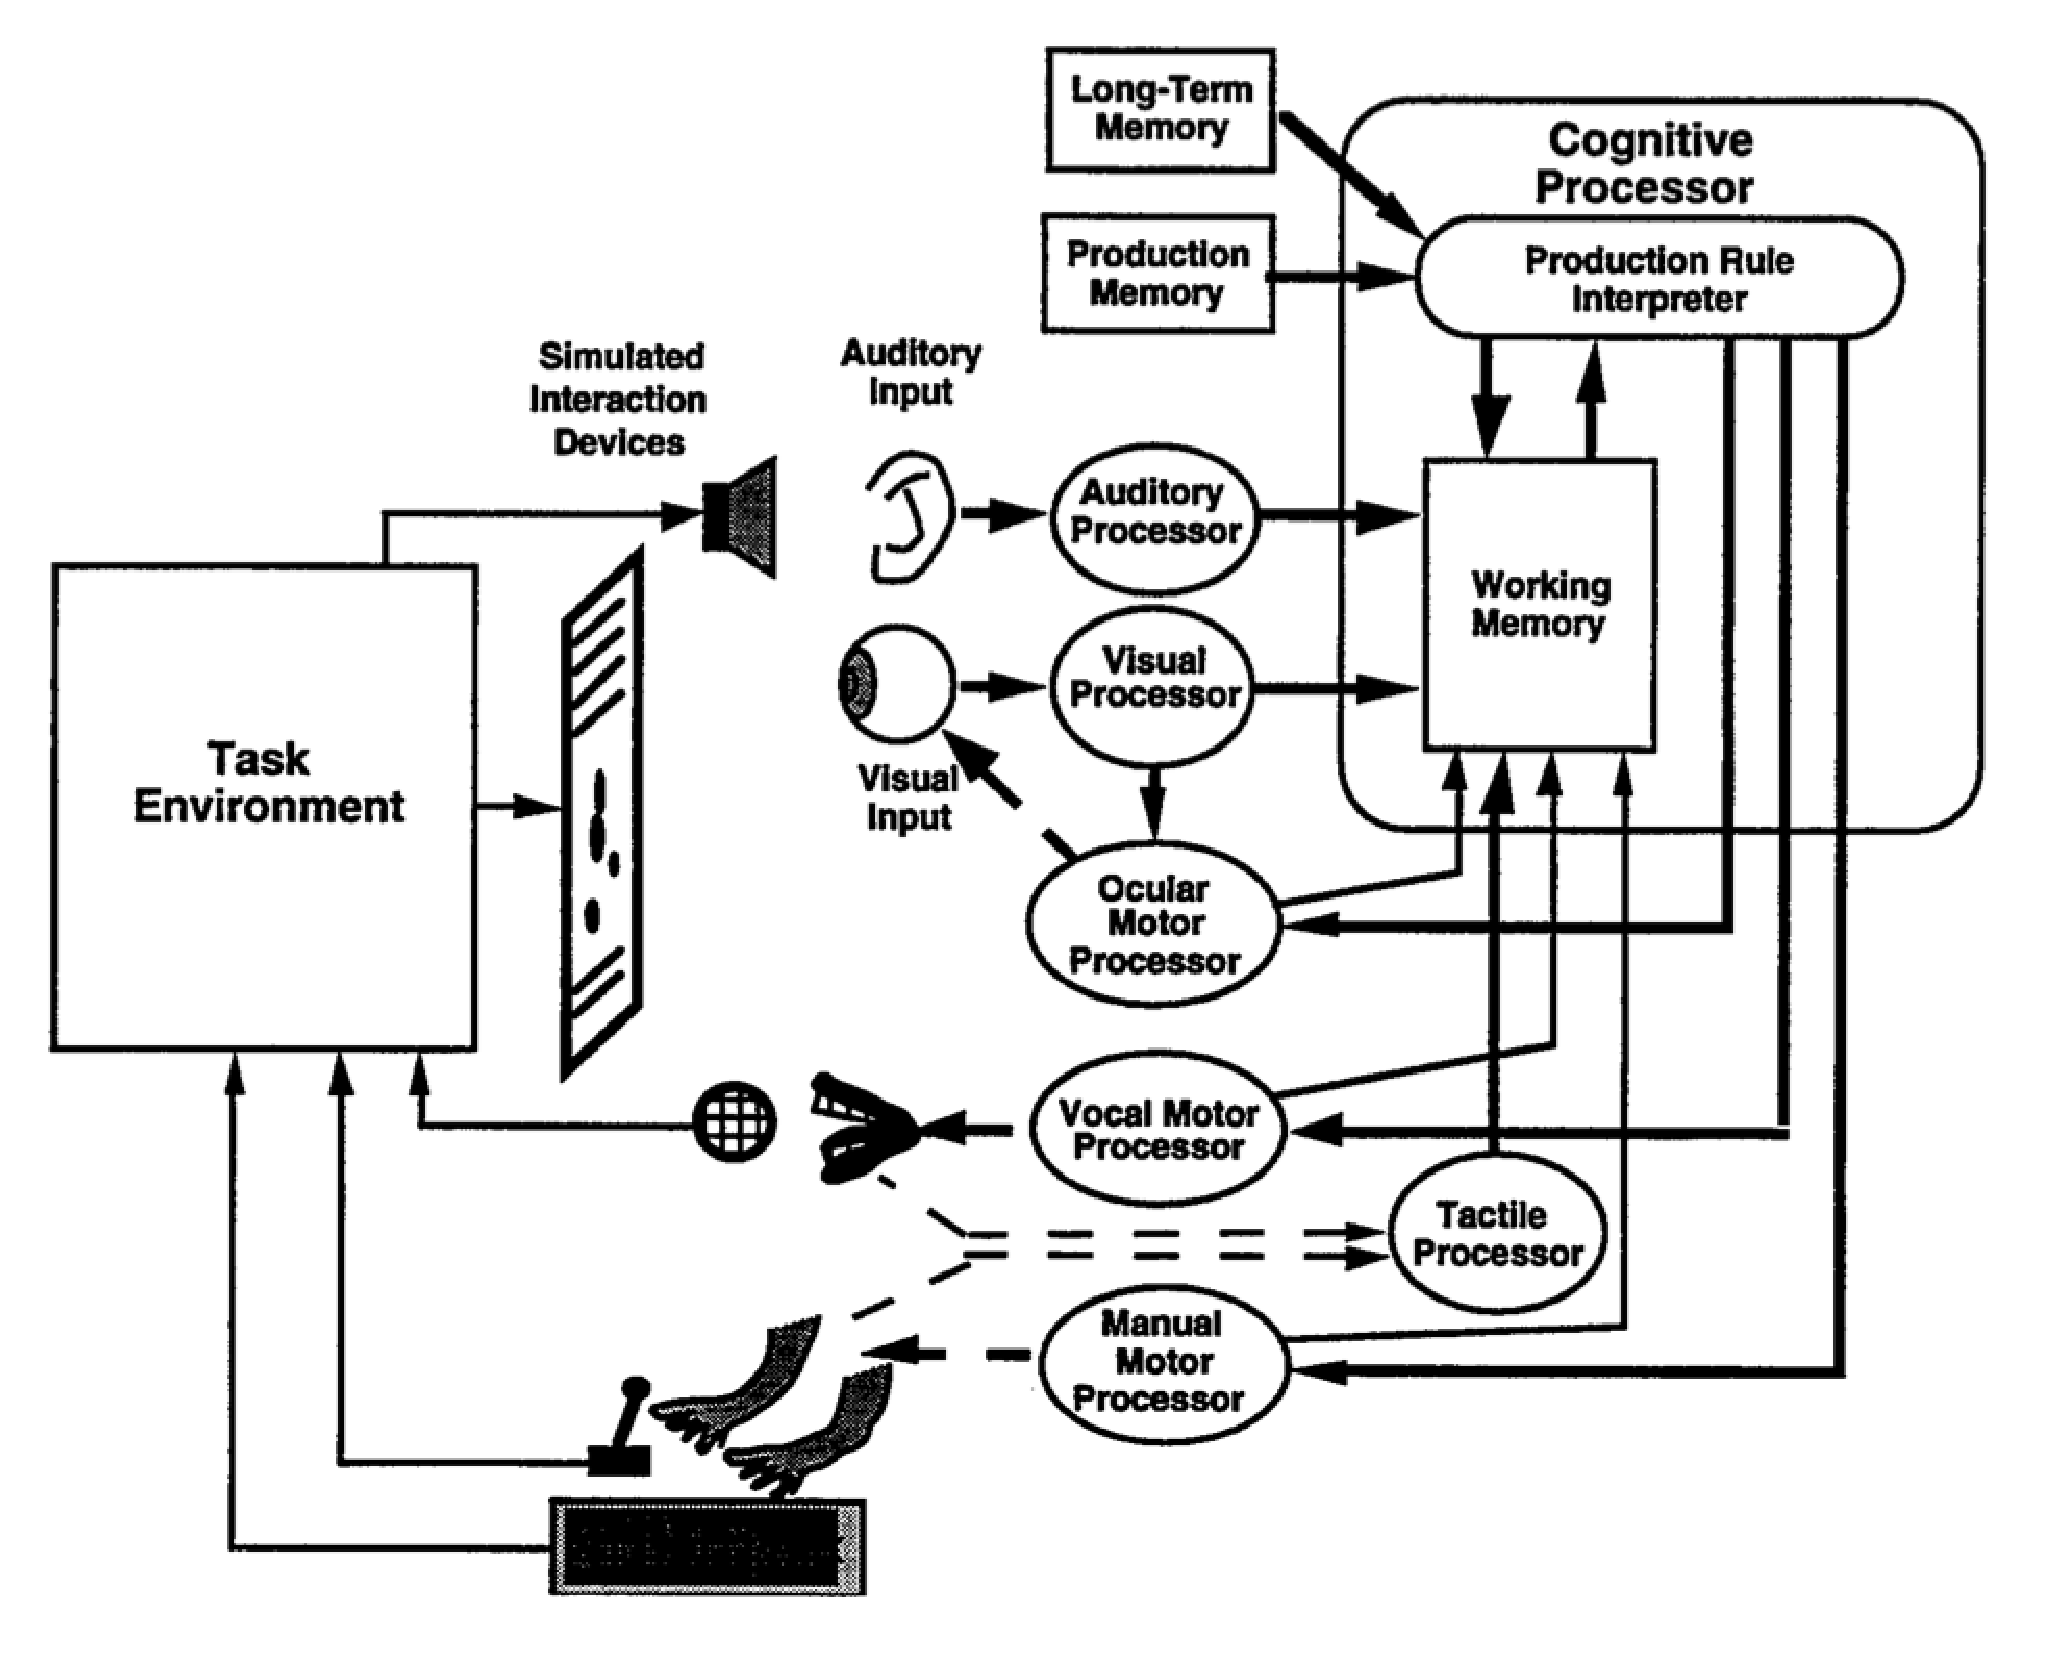
\includegraphics[width=100mm]{EPIC.eps}
  \caption{The architecture of EPIC\cite{citeulike:3439185}}
  \label{EPIC_ARCH}
\end{figure}
%   Mechanics of cognition
%      Means of planning, Learning
Like \soar, the \epic architecture executes its productions in the
form of a decision cycle, where each cycle lasts for a period of
50 milliseconds. The cycle starts with obtaining inputs from its perceptual
processors. The production system then fires all productions whose
conditions match the contents of working memory.  All their
corresponding actions are executed. The actions of the action items
are restricted to adding and removing items from the working memory
and to send commands to the motor processor.

%   Abilities of perception
%      Auditory, Visual
The \epic architecture models perceptual and motor facilities with
good accuracy. The perceptual and motor modules that interface with
the world are known as processors. Both the perceptual and the motor
processors can function in parallel. Perceptual processors simulate
the working of human perceptual facilities: these include visual
processors and auditory processors. The motor processors deal with
performing actions that affect the environment: some examples of motor
processors are the manual motor processor, the vocal motor processor,
and the oculomotor processor.

The visual processor is used to identify visual objects in the
environment. The visual processor maintains information which objects
are visible and what their properties are. The auditory processor
accepts auditory input and outputs a representation of auditory
events. These events fade away after a period of time (4 seconds). To
represent the sequential order of speech, the auditory processor adds
tags to the inputs in sequence to indicate temporal relationships
between words.

The motor processors require two distinct phases to execute a motor
command, the preparation phase and the execution phase. The
preparation phase involves compiling the commands from the cognitive
processor into a set of features that characterize the movement. The
execution phase begins after the preparation phase has completed. The
movement features remain in the processor's memory.  As a result
future movements that perform the same action are performed
faster. The manual processor represents physical movements like
pressing keys, moving fingers and hands to another location, and so
forth. The vocal motor processor is used to create utterances of
speech. The oculomotor processor controls the movement of the eyes.

\subsection{CLARION}
% General background
\clarion (Connectionist Learning with Adaptive Rule Induction ON-line)
\cite{journals/cogsci/SunMP01} was developed with two major
motivations. 

\begin{itemize}
\item \emph{Study of low-level skill acquisition}: Sun
  et al.~\cite{journals/cogsci/SunMP01} concentrate on low-level cognitive
  skills in \clarion.  They cite reactive
  sequential decision making as an instance of low-level cognitive
  skill. In such a task the agent would have to pick an action to
  achieve an objective based on the information available at a
  given point in time.
\item \emph{Model learning that does not require a large amount of
    priori knowledge}: Sun et al. state that the process of learning
  in situations where agents are given the required amount of
  knowledge which they convert into procedural skill is considerably
  different from a situation where the agent is not provided with
  enough {\em a priori} knowledge. The authors suggest that in such
  cases the learning that occurs is of ``bottom-up'' nature.
\end{itemize}

\begin{figure}[htp]
  \centering
  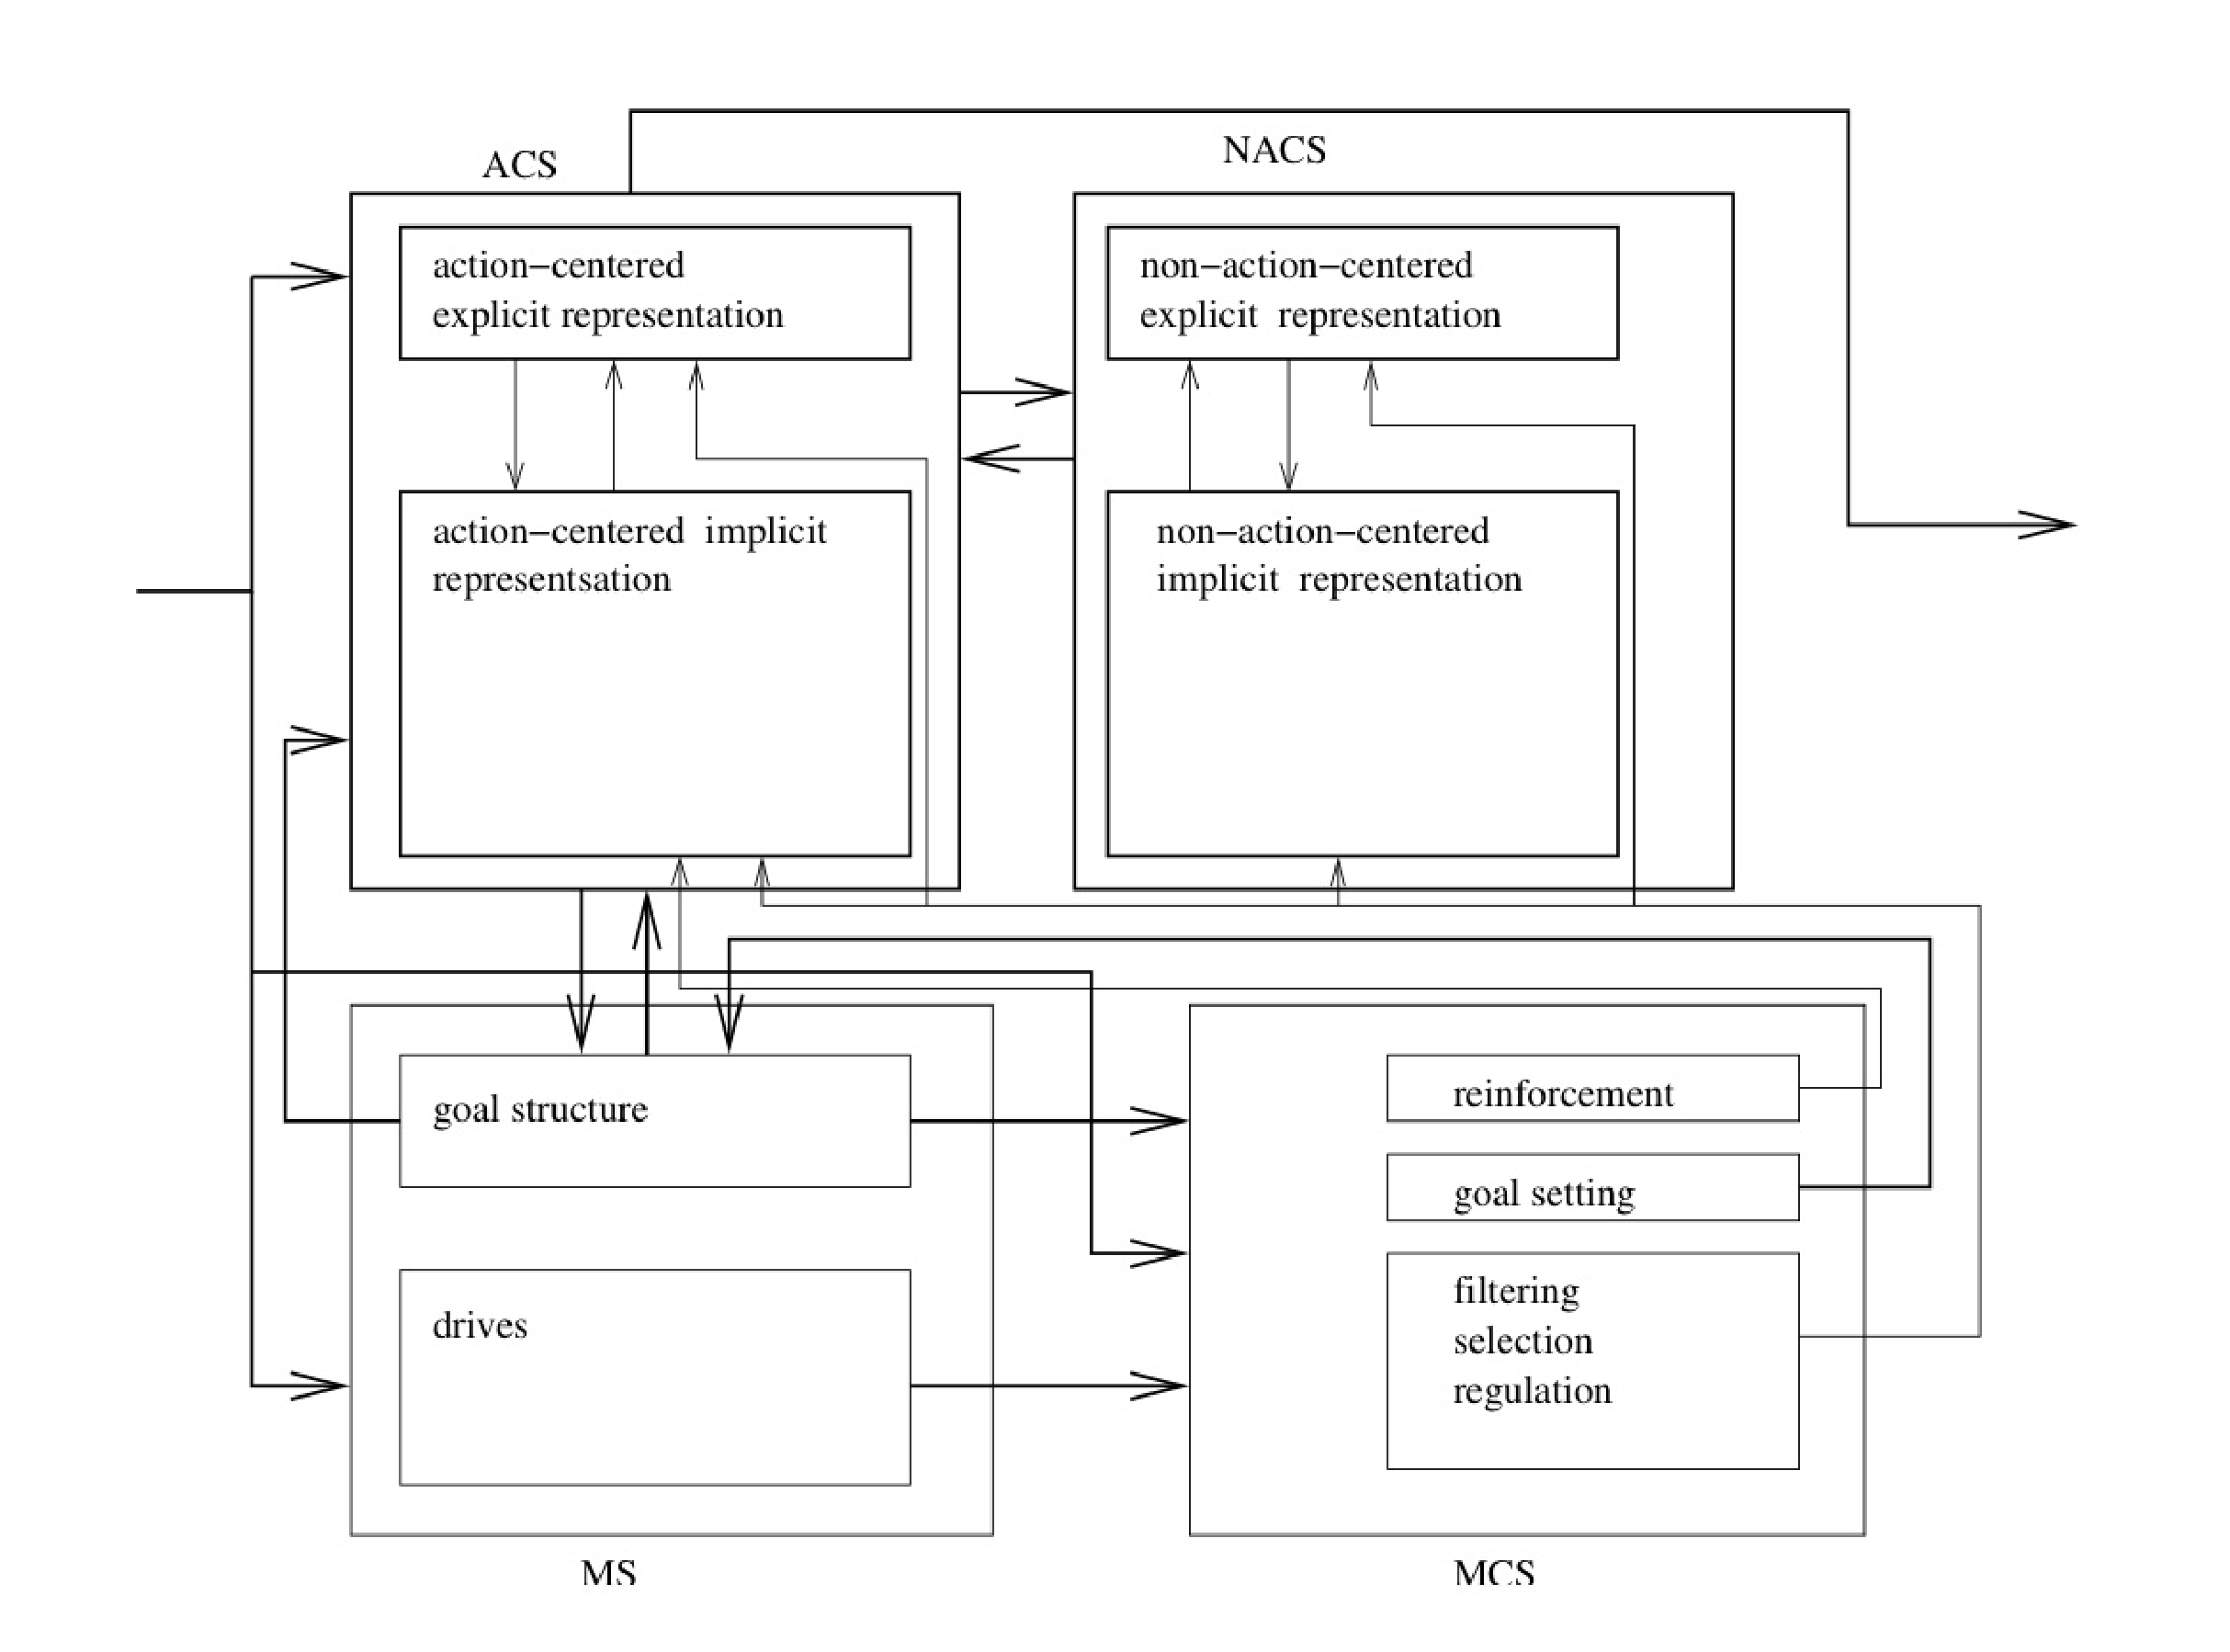
\includegraphics[width=110mm]{CLARION.eps}
  \caption{The architecture of \clarion~\cite{citeulike:3439185}}
  \label{CLARION_ARCH}
\end{figure}

% Describe architecture 
Research with \clarion advocates that cognitive systems are two-level
architectures.  A top level encodes explicit knowledge
such as production rules, explicitly specified prior knowledge. The
lower level is used to store implicit knowledge, such as memory
associations, in the form of neural networks. \clarion consists of four
major subsystems.  These are described below; the schematic of the same
can be seen in Figure~\ref{CLARION_ARCH}.
% This system cannot be described in the given format, it makes sense
% to

The action-centered subsystem is perhaps the most important component
of the system. Its functions include calculating the quality of
various actions given the current scenario, choosing an appropriate
action for the situation, performing the action, and observing the
change in the state.  Updates are made to the internal representation
during this process, including changes to the rule network (shown in
the upper level of the action centered subsystem) using a rule
extraction and refinement algorithm. The lower level of the
action-centered subsystem also holds sensory information, working
memory items, and information from the goal
structure~\cite{Sun:2003aa}.

The Non-Action-Centered subsystem is used to represent general
information about the real world. A back propagation algorithm is used
to establish relationships between various pairs of inputs and
outputs. The Non-Action-Centered subsystem can also apply
similarity-based reasoning in addition to associative rules.

Real-world cognition is driven by the environment around an agent, but
it also depends on the underlying motivation of the agent. With
\clarion, Sun et al. also study the underlying motivations that drive
the actions an agent intends to achieve. This area of cognition is
modeled and studied using the Motivational and Meta-Cognitive
subsystems.  These subsystems explain, for example, what makes one
course of action or cognitive processing more attractive than another.

\subsection{Criteria for comparison}
This section provides a comparison of various integrated cognitive
architectures on various parameters, shown in
Table~\ref{tab:architecture-comparison}. The parameters have been
selected based on the work of Anderson and
Lebiere~\cite{CambridgeJournals:207162}.

\begin{sidewaystable}[h]
  \centering
\caption{Comparison of various cognitive architectures}
\label{tab:architecture-comparison}
  \begin{tabular}{p{3cm}p{4cm}p{4cm}p{4cm}p{4cm}}
  \hline
  Parameters & ACT-R & EPIC & SOAR & CLARION \\
  \hline
  & & & &\\
  Representation of knowledge in memory & Knowledge represented as chunks. Memory consist of a
  working memory and long term memory.& Long term and short term
  memory where information was stored as productions in long term
  memory & Knowledge in both the short term and long term memory
  represented as production rules& Procedural at the bottom level and
  declarative at the top  \\
  & & & &\\
  Goals  & Maintained by the goal buffer & Priority based task
  deferment~\cite{Pew:1998aa}& Represented as states & Goal stack or list \\
  & & & &\\
  Problem Solving  & Based on selection and execution of production
  and the underlying neural network.& Problem solving based on &Search
  of the solution space& Combination of calculated Q-Values and rules\\
  & & & &\\
  Planning  & Creation of sub-goals&General planning & Selection of
  productions that leads the system closer to achieving its
  goals. &Search through the Q-Value space \\
  & & & &\\
  Learning   & Production compilation&No learning & Learning through
  chunking & Reinforcement learning and rule extraction \\
  & & & &\\
  Perception & Provides vision and auditory faculties through the
  relevant buffers& Perceptual processors for auditory, visual and
  tactile faculties & (No explicit commitments.) & Input in terms of dimension/value pairs\\
  & & & &\\
  Motor & Provides motor control through the manual and vocal modules&
  manual, vocal and oculo-motor processors
  & (No explicit commitments.) &\\
  & & & &\\
  Mapping to the brain$<$Select better name$>$ & Study currently on
  that maps regions of the brain to specific modules& No mapping& No
  mapping& based on neural network but no reference to the brain anatomy\cite{Chong:2007aa} \\
  & & & &\\

\end{tabular}
\end{sidewaystable}

% Things to be concerned about
%    Type of system: Symbolic, Connectionist or both
% 1) Perception: How an architecture gets its input
% 2) Memory: How is memory represented
% 3) Goals: How goals are represented and solved
% 4) Problem Solving: Techniques for solving problems
% 5) Planning: Planning techniques used 
% 6) Reasoning: How do system reason
% 7) Learning: How stuff is learnedn
% 8) Meta Processing: ??
% 9) Natural language processing: How is natural language processed
% 10) Query Answering: Not required
% 11) Diagnosis: Not required
% 15) Ability to recover from failure
% 18) Reusability
% 19) Mapping to the brain

%\vspace{5cm}

\section{Challenges facing cognitive architectures}

%Summarise this section
This section provides a brief, general summary of limitations
of attempts to model human cognition.
%
% It also surveys a number of cognitive architectures and attempts to
% provide a brief overview of the state of the art in the area of
% cognitive architectures.
%
% Say though all this work there are still some open issues, cite the
% paper and describe the issues.
Despite the tremendous amount of effort that has gone into this area, we
are nowhere near the end. There are a number of research questions
that are open for curious minds to explore. These areas are spelled
out clearly by Langley et al.~\cite{citeulike:4182324}:

\begin{itemize}
\item \emph{Architectures need to explore categorization and
    understanding}: Currently cognitive architectures have not paid
  significant attention to the means by which we understand concepts
  and ideas. This is also the case with categorization, the ability of
  humans to categorize object that may seem dissimilar at first.
  
\item \emph{Accurately reflecting perceptive abilities of physical
    agents}: Most architectures tend to ignore the fact that a human
  has limited abilities to gather information relevant to a given
  task. Architectures need to replicate this behaviour if we are to
  acquire a greater understanding of human cognition.

% People Need to focus more on episodic knowledge
\item \emph{Further emphasis on episodic memory}: Episodic memory is a
  form of declarative memory that requires context and personal
  participation\cite{09011999}; for example, the memory associations
  of one person's eighteenth birthday may be completely different from
  those of another.  The focus on problem solving and skills has
  distracted cognitive architecture researchers from studing the
  complete nature of episodic memory.

% Extend frameworks to build knowledge formalisms to enable
% intelligent behaviour
\item \emph{Further study of knowledge representation}: Humans rely on
  a number of ways of representing knowledge using visual or auditory
  representations.  This stands in contrast to most cognitive
  architectures, which have essentially been tied down to representing
  knowledge in the form of production rules or similar forms. There
  must be further study of different representational schemes that can
  be used (e.g., a more flexible frames-based
  approach~\cite{Minsky1974a} or description
  logics~\cite{nardi-brachman:2003a}).
%\textsc{REUBEN:TODO:get a background    on description logics}

% No cognitive architectures handle interaction between body and mind.
\item \emph{Study of body-mind interaction}: Despite the large number
  of topics addressed in cognitive architecture reseach, the area of
  body-mind interaction has not been explored in detail.

% Emotions, no architectures handle that

\item \emph{Study of emotion}: Emotions are arguably what define
  humans and in quite a few cases determine their choices.  Cognitive
  science and cognitive architecture research needs to explore this
  area to get a more complete picture of human cognition.

% use natural language processing more
% \item \emph{Farther the use of natural language:} Cognitive
%   architectures have done a considerab
% This point does not hold, because I would rather have raw data on
% which I would be able to run a whole lot of metrics rather than
% having any other sort of output.
% REUBEN:TODO:Speak to prof about this.


\end{itemize}

%This is more of an engineering point of view, the idea is that most
%cognitive architectures do not support reuse as a part of the
%them. This project is a step in exploring how models can be shared
%and reused.

The challenges described above are conceptual, but they also have an
engineering component.  From an engineering standpoint, a cognitive
modeller essentially builds intelligent agents by writing programs
within a framework that postulates a theory of cognition. There are
situations where a similar task may be modeled by one or more
researchers.  In the current state of affairs, collaboration happens
by a variety of informal and opportunistic ways.  This results in
duplication of effort and, in some cases, work that might be improved
if tighter collaboration had been possible.  The aim of this project
is to take a step toward improving this situation.

% Quicker development times
% Lesser bugs
% Greater coherence
% Areas can be explored more thoroughly because creating models is
% easy and cheap
% Sharing knowledge and resource